\begin{blocksection}
\question Is this algorithm for computing the shortest path between two
vertices correct?

Given a starting vertex, $s$, and an ending vertex, $v$, compute the shortest
path between $s$ and $v$ by running DFS, but at each node exploring the
shortest outgoing edge first until $v$ is reached. Return the $s$ to $v$ path
in the DFS tree.

\begin{solution}[2in]
Incorrect. Consider the graph below whose true shortest path is $s - v$ but
whose greedy DFS path is $s - t - v$.

\begin{center}
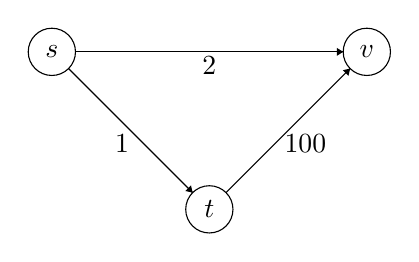
\begin{tikzpicture}[scale=0.1]
\tikzstyle{every node}+=[inner sep=0pt]
\draw (20,-20) circle (3);
\draw (20,-20) node {$s$};
\draw (60,-20) circle (3);
\draw (60,-20) node {$v$};
\draw (40,-40) circle (3);
\draw (40,-40) node {$t$};
\draw (22.12,-22.12) -- (37.88,-37.88);
\fill (37.88,-37.88) -- (37.67,-36.96) -- (36.96,-37.67);
\draw (28.92,-30.48) node [below] {$1$};
\draw (42.12,-37.88) -- (57.88,-22.12);
\fill (57.88,-22.12) -- (56.96,-22.33) -- (57.67,-23.04);
\draw (52.2,-30.48) node [below] {$100$};
\draw (23,-20) -- (57,-20);
\fill (57,-20) -- (56.2,-19.5) -- (56.2,-20.5);
\draw (40,-20.5) node [below] {$2$};
\end{tikzpicture}
\end{center}
\end{solution}
\end{blocksection}
